\chapter{Calculus}

\section{Set Theory}
The elements of a set can be chosen abstractly. For instance, in a university, a set of people can contain students, teachers, and faculty. We denote the objects of the set as generalized things. For instance, numbers, animals, and personal emotions are all things that we can place in a set.

Denote the set by the curly-brackets $\{\}$. The following operations all

\begin{definition}
    \begin{itemize}
        \item Let $\cup$ define set union. Ie, if $x \in A, y \in B, \{x,y\} \in A\cup B$.
        \item Let $\cap$ define set intersection. This is defined as if $x, y \in A\cap B$, then $x \in A, x\in B, y\in A, y\in B$.
        \item Let $A$ be a set. Let $B$ be a subset of $A$, that is, $B\subset A$.  Then, let $B^c$ denote the compliment of $B$, or the points in $A$ that are not in $B$. If $A = B$, then $B^c = \emptyset$.
    \end{itemize}
\end{definition}

We can use these operations to discuss some interesting groups of numbers. The following are a few useful sets.

\begin{definition}
    The following are commonly used sets;
    \begin{itemize}
        \item Natural numbers: $\mathbb{N} = \{1,2,3,\dots \}$ 
        \item Whole Numbers: $\mathbb{W} = \{0, 1,2,3,\dots \}$
        \item Integers:$\mathbb{Z} = \{\dots, -3, -2, -1, 0, 1,2,3,\dots \}$
        \item Rational Numbers: $\mathbb{Q} = \left\{\frac{x}{y} : \{x,y\} \in \mathbb{Z}, y\neq 0\right\}$
        \item Irrational Numbers: $\mathbb{P} = \left\{x : x\text{ cannot be written as a fraction.}\right\}$
        \item Real Numbers: $\mathbb{R} = \mathbb{Q}\cup \mathbb{P}=\mathbb{Q} \cup \mathbb{Q}^c$
    \end{itemize}
\end{definition}

\subsection{Properties of Set Operations}
The operations of set union and intersection allow us to learn about the properties of sets under union, intersection, and compliment. We can define a few interesting theorems or results that allow us to start getting some logic in the world. 

\begin{theorem}
    \begin{equation}
        X^c \cap Y^c = (X \cup Y)^c
    \end{equation}
    \begin{proof}
        To prove this, we need to show that the LHS is equal to the RHS. Consider $X \cup Y$. If $x\in X^c$ then $x \notin X$. If $y\in Y^c$, $y\notin Y$. The overlap of the compliment sets, $X^c \cap Y^c$, contains neither $x$ nor $y$. Thus, $x, y \in X\cup Y$, This completes the proof as since $x,y \notin X^c \cap Y^c$, then we must have that $(X\cup Y)^c = X^c \cap Y^c$.
    \end{proof}
\end{theorem}

For a union or intersection of many sets, define the notation;
\[
\bigcup_{i=1}^\infty X_i = X_1 \cup X_2 \cup \dots, \quad \bigcap_{i=1}^\infty X_i = X_1 \cap X_2 \cap \dots
\]

\begin{theorem}
    \begin{equation}
            \left(\bigcap_{i=1}^\infty X_i\right)^c =     \bigcup_{i=1}^\infty X_i^c 
    \end{equation}
    \begin{proof}
        Let $x_i \in X_i$, $x_i\notin X_i^c$. Split this into two cases, where $\cap X_i \neq \emptyset$ and $\cap X_i = \emptyset$. 
        \begin{itemize}
            \item $\cap X_i = \emptyset$, then for every $x_i$ there exists a disjoint set $X_j$ which doesn't contain $x_i$. This implies that $x_i \in X^c_j$.
            \item $\cap X_i \neq \emptyset$. If the intersection is not empty, then there exists $x_i \in X_1, X_2, \dots$. Thus, since $x_i$ is simultaneously contained within every intersected set;  $x_i \notin \cup X_i^c$.
        \end{itemize}
        This completes the proof stating that the compliment of the intersection of all sets will contain all points outside of the intersection which is the union of each individual compliment. 
    \end{proof}
\end{theorem}

\subsection{Functions}

We can furthermore define functions as sets by adressing rules. Depending on these rules, a function can map an element in set $A$ to set $B$. This is defined using the following notation;
\begin{equation}
    f : A \rightarrow B
\end{equation}

\begin{example}
    Suppose $f(x) = 3x^2$ for $x\in \mathbb{R}$. Define the set $\mathbb{R}_+ = [0, \infty)$. Thus, we would say that;
    \begin{equation}
        f: \mathbb{R} \rightarrow \mathbb{R}_+
    \end{equation}
\end{example}

We can classifty functions based on the uniqueness of their mappings. For a function $f: A \rightarrow B$, we assume that each element in $A$ maps to at most one element in $B$. A general function takes an element in $A$ and maps to at most one value in $B$. Not all elements need to be mapped to, and some points can be visited multiple times. \textbf{Injectivity} implies that each input on $A$ produces a unique result in $B$. Ie, there are no duplicates. However, not all elements in $B$ are nessecarily covered. \textbf{Surjectivity} implies that all outputs in $B$ are mapped to, however, multiple $x\in A$ may map to elements in $B$. A map is \textbf{bijective} if every point in $A$ uniquely maps to a point in $B$. This is also known as a set which is injective and surjective. See Fig. \ref{fig:bijective} for a visualization.

There are some useful notation. Here, for $f:X \rightarrow Y$, define the \textbf{image} as the set $Y = f(X)$. similarily, define the inverse image, or \textbf{preimage} as the set $X = f^{-1}(Y)$. 

\begin{figure}[htbp!]
    \centering
    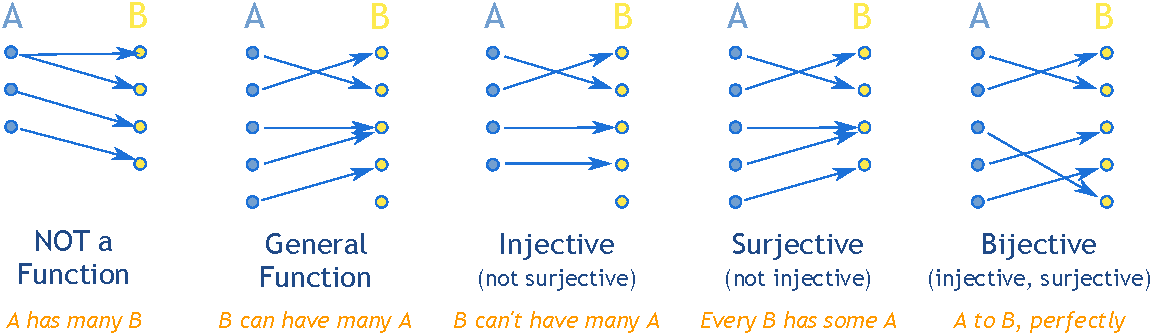
\includegraphics[width=\textwidth]{figures/set_theory/function-mapping.pdf}
    \caption{Function types based on correspondance. For a function $f: A \rightarrow B$, we assume that each element in $A$ maps to at most one element in $B$. A general function takes an element in $A$ and maps to at most one value in $B$. Not all elements need to be mapped to, and some points can be visited multiple times. \textbf{Injectivity} implies that each input on $A$ produces a unique result in $B$. Ie, there are no duplicates. However, not all elements in $B$ are nessecarily covered. \textbf{Surjectivity} implies that all outputs in $B$ are mapped to, however, multiple $x\in A$ may map to elements in $B$. A map is \textbf{bijective} if every point in $A$ uniquely maps to a point in $B$. }
    \label{fig:bijective}
\end{figure}

\begin{definition}
    general functions have the following properties when used in tandem with set union and intersection. In addition, we present the inverse operations. 

    \begin{enumerate}[label=\alph*.]
        \item $f(A\cup B) = f(A) \cup f(B)$
        \item $f(A\cap B) \subseteq f(A) \cap f(B)$
        \item $f^{-1}(A\cup B) = f^{-1}(A) \cup f^{-1}(B)$
        \item $f^{-1}(A\cap B) = f^{-1}(A) \cap f^{-1}(B)$
        \item $f^{-1}(f(A)) \supseteq A$
        \item $f(f^{-1}(C)) \subseteq C$
    \end{enumerate}
\end{definition}
\begin{proof}
    We aim to prove each statement mentioned above. Let $f:X \rightarrow Y$ and $A, B\subset X$, $C\subset Y$. 
    \begin{enumerate}[label=\alph*.]
        \item  Let $x\in f(A\cup B)$. Thus, there exists a $y$ such that $y \in A\cup B \rightarrow x \in f(y)$ Since $y\in A, \rightarrow x \in f(A)$ or $y\in B \rightarrow x \in f(B)$. Thus, $f(A\cup B) \subseteq f(A) \cup f(B)$. Similarily, in the converse, suppose that $x\in f(A)$. then, there will exists a $y\in A$. Since $y \in A, y\in (A\cup B)$. Thus, $f(A) \subseteq f(A\cup B)$. Or more relevantly, $f(A) \cup f(B) \subseteq f(A\cup B)$. The converse with $B$ is trivial. Thus,  $f(A\cup B) = f(A) \cup f(B)$.
        \item Let $x\in f(A \cap B)$. There exists a $y$ such that $y\in A$ and $y\in B$, so $y \in A\cap B$. So, if $y\in A$, $x\in f(A)$ and $y\in B$, $x\in f(B)$. If both are true simultaneously, then $f(A\cap B) \subseteq f(A) \cap f(B)$. 
        \item Assume that $x \in f^{-1}(A\cup B)$ Then, $f(x) \in A \cup B$. Since $f(x) \in A$ and $f(x) \in B$ and for all $A, B$ there exists a preimage, then $f^{-1}(A\cup B) \subseteq f(A) \cup f(B)$. The second inclusion is shown by the converse. Let $x\in f^{-1}(A) \cup f^{-1}(B)$. Since $f(x) \in A \cup B$ then $f^{-1}(A) \cup f^{-1}(B) \subseteq f^{-1}(A\cup B)$. Both inclusions are true, so there is an equality.
        \item Let $y \in f^{-1}(A\cap B)$ such that $f(y) \in A \cap B$. So, $f(y) \in A$ and $f(y)\in B$. Thus, $y \in f^{-1}(A)$ and $y \in f^{-1}(B)$. Or $y\in f^{-1}(A) \cap f^{-1}(B)$. So, $f^{-1}(A\cap B) = f^{-1}(A) \cap f^{-1}(B)$.
        \item Let $x \in f^{-1}(f(A))$. The inverse image of $f(A)$ will point to $A$ if $f$ is injective. Otherwise, it is at most a subset of $A$. $f^{-1}(f(A)) \supseteq A$ 
        \item Let $x \in f(f^{-1}(A))$. The image of the preimage is the identity if every element in $A$ is mapped to. Thus, the identity is equal if $f$ is surjective. 
    \end{enumerate}
\end{proof}

Remark that if $f$ is a bijective map, then $f^{-1}(f(A)) = f(f^{-1}(A))$. 

\clearpage
\subsection{Problems}
\begin{problem}
    Let $\leq, \geq$ have their regular definitions. Let $A = \{0\leq x \leq 3, x \in \mathbb{R}\}, B = \{-1\leq x \leq 1, x \in \mathbb{R}\}$. Show that $A\cap B = C = \{0\leq x \leq 1, x \in \mathbb{R}\}$
\end{problem}

\begin{solution}
    To show this, we need to show that the LHS is equal to the RHS for the final line in the problem statement.  Trivially, $C \subset A$; $\inf C \in A, \sup C \in A$. Thus, $\forall x \in C, x \in A$. Similarily, $C \subset B$ by the same logic. Thus, state $C^c = (-\infty, 0) \cup (1, \infty)$. Furthermore, writing the union of elements in the compliments of $A, B$; $A^c \cup B^c = (-\infty, 0) \cup (1, \infty)$. We use the property of intersections of sets 
    \begin{align*}
        A^c \cup B^c &= (A \cap B)^c \\
                  C^c  &= (A \cap B)^c \\
                  C &= A \cap B
    \end{align*} 
    $\blacksquare$
\end{solution}

\begin{problem}
    List elements of;
    \begin{equation}
        \left(\{2,3,4\} \cup \{x\in \R: x^2 -4x +3 = 0 \}\right) \cap \{x\in \R:-1 \leq x < 3\}
    \end{equation}
\end{problem}
\begin{solution}
    The LHS of this contains two sets. The right-set are solutions to a quadratic equation. This contains two elements. 
    \[
    x_{1,2} = \frac{4 \pm \sqrt{16 - 12}}{2} = \{1, 3\}
    \]
    Thus, the LHS is the union of two sets. Rewriting this;
    \begin{equation}
       \{1,2,3,4\} \cap \{x\in \R:-1 \leq x < 3\}
    \end{equation}
    The intersection of the discrete set of integers between 1 and 4 and the open neighborhood between -1 and 3 is simply $\{1, 2\}$ as 3 is not included in the set. 
    \begin{equation}
        \left(\{2,3,4\} \cup \{x\in \R: x^2 -4x +3 = 0 \}\right) \cap \{x\in \R:-1 \leq x < 3\} = \{1,2\}
    \end{equation}
\end{solution}

\begin{problem}
    If $A \subset S$, show the following;
    \begin{enumerate}[label=\alph*.]
        \item  $(A^c)^c = A$
        \item $A\cup A = A\cap A = A \cup \emptyset = A$
        \item $A \cap \emptyset = \emptyset$
        \item $A \times \emptyset = \emptyset$
    \end{enumerate}
\end{problem}

\clearpage
\section{The Real Number System}

The real numbers are defined by a set of axioms. There are various ways to treat this. I am going to just state all of the properties upfront and then proceed with the consequences of their existence. 


\begin{theorem}
    \label{thm:realnumber}
    \textbf{Axioms of the Real Number System:} These are the axioms that define the set of real numbers. The properties are stated outright, then the consequences are listed in further statements.
   
    \begin{enumerate}[label=F\arabic{*}:]
        \item \textbf{Commutativity}; Let $a, b \in \R$, then $a + b = b + a$, and $a \cdot b = b \cdot a$. 
        \item \textbf{Associativity}; Let Let $a, b, c \in \R$, then $(a + b) + c = a + (b + c)$, and $a \cdot (b \cdot c) = (a\cdot b) \cdot c$.
        \item \textbf{Distributitivity}; $a \cdot (b + c) = ab + ac$
        \item \textbf{Existence of Neutral Numbers}; $a + 0 = a$, $a \cdot 1 = a$
        \item \textbf{Existence of Additive and Multiplicative Inverse Numbers}; For any $a 
         \in \R$ there exists a number $b$ such that $a + b = 0$, where $b = -a$. Simiarily, there exists a number $c$ such that $a \cdot c = 1$, where $c = a^{-1}$.
    \end{enumerate}
    \begin{enumerate}[label=O\arabic{*}:]
        \setcounter{enumi}{5}
        \item \textbf{Order}; There is a subset of $\R$ known as $\R_+$ such that the two properties are satisified:
        \begin{itemize}
            \item If $a, b \in \R_+$, $a + b \in \R_+$, $a \cdot b \in \R_+$. 
            \item For any $a \in \R$ only one of the following is true. \[a\in \R_+,\quad a = 0,\quad -a \in \R_+\]. 
        \end{itemize}
        The numbers such that $a \in \R_+$ are known as positive numbers, while the numbers such that $-a \in \R_+$ are known as negative numbers. 
    \end{enumerate}
    \begin{enumerate}[label=LUB\arabic{*}:]
        \setcounter{enumi}{6}
        \item \textbf{Least Upper Bound}; A nonempty set of real numbers that is bounded from above will have a least upper bound. 
    \end{enumerate}
\end{theorem}

The real number system is completely defined by the Thm. \ref{thm:realnumber}. We can now form the properties and rules of algebra on the real number system. 

\begin{enumerate}
    \item In a sum or product of many numbers, the parentheses can be omitted; $(a + (b + c)) + d = a + ((b + c) + d) = (a + b) + (c + d) = \dots$ by F1 and F2.
    \item  In a product of many numbers, order is immaterial; $a \cdot b \cdot c = b \cdot a \cdot c = c \cdot a \cdot b = \dots$
    \item For any $a,b \in \R$ the equation $x + a = b$ has one and only one solution. For, if $x\in \R$ then see the following computation.
    \begin{align*}
        x &= x + 0\\
        &= x + ((a) + (-a))\\
        &= (x + a) +(- a)\\
        &= b + (-a) \\
        x &= b + (-a)
    \end{align*}
    Thus, $x = b + (-a)$ is the only solution.
    \item For any $a,b \in \R$, with exception $a\neq 0$ the equation $xa = b$ has one and only one solution.
    \begin{align*}
        x &= xa a^{-1} \\
        &= (x a) \cdot a^{-1} \\
       x &= b a^{-1} 
    \end{align*}
    Thus, the element 1 is unique from F4. we define $a^{-1} = \frac{1}{a}$

    \item For any element $a\in R$, $a \cdot 0 + a \cdot 0 = a\cdot (0 + 0) = a \cdot 0 = a \cdot 0 + 0$. So both $a \cdot 0$ and $0$ are solutions of the equation $x + a \cdot 0 = 0$. Thus, if a product of numbers is 0 then at least one of the element must be 0. for if $ab = 0$ and $a\neq 0$ then we can multiply both sides by $a^{-1}$ to get $b = 0$. Hence, the illegitimacy of division by 0. 
    \item Solutions of the equation $x + (-a) = 0$ are given by $-(-a)$ given by (3.). By F5, we have $-(-a) + (-a) = 0$, so $-(-a) = a$ for any $a \in \R$.
    \item $(a^{-1})^{-1} = a$ for any non-zero $a \in \R$.  Since $a \cdot a^{-1} = 1$ by F5,  and we know that $a^{-1} \neq 0$, then F4 implies that  $(a^{-1})^{-1}$ and $a$ are equal as both are solutions to $x + a^{-1} = 1$.
    \item $-(a+b) = (-a) + (-b)$ for all $a,b \in \R$ as both are solutions to the equation $x + (a + b) = 0$. 
    \item $(ab)^{-1} = a^{-1} b^{-1}$ for any $a,b \in \R$, $a,b \neq 0$. Both are solutions to the equation $x(ab) = 1$. 
    
    From this, we can define the rules of the fraction;
    \begin{align*}
        \frac{ac}{bc} &= ac (bc)^{-1} = ab^{-1} c c^{-1} = ab^{-1} = \frac{a}{b} \\
        \frac{a}{b} \cdot \frac{c}{d} &= ab^{-1} c d^{-1} =ac (bd)^{-1} = \frac{ac}{bd} \\
        \frac{a}{b} + \frac{c}{d} &= ab^{-1} + cd^{-1} =ab^{-1}d d^{-1} + c b b^{-1} d^{-1} \\
        &= (ad + cb) \cdot (b^{-1} d^{-1}) = \frac{ad + cb}{bd}
    \end{align*}
    \item $a \cdot (-1) = -a$ for all $a\in \R$. Since $(-1) \cdot a + a = a((-1) + 1) = a \cdot 0 = 0$. We have that $(-1) \cdot a$ and $a$ are solutions to the equation $x + a = 0$, hence are equal. 
    
    A consequence of this is that $-a \cdot b = (-1) \cdot a \cdot b = -ab$ and $(-a) \cdot (-b) = (-1) \cdot (-1)\cdot  a\cdot b = ab$
\end{enumerate}

These are the field properties of the real numbers and apply to fields such as the rational and complex numbers. To define the reals, The order and LUB properties need to be applied. We can now discuss the order properties of the real numbers. 

\begin{enumerate}
    \item If $a,b \in \R$ only one of the following statements is true;
    \begin{align*}
        a &< b \\
        a &= b \\
        a &> b \\
    \end{align*}
    This is the case as we apply $(a-b)$ then the number must fit in one of three subsets, being $a\in \R_+, -a \in \R_+, a\in \{0\}$.
    \item if $a >b$ and $b>c$ then $a-b \in \R_+$ and $b - c\in R_+$. Thus, $a - c = (a-b) + (b-c) \in \R_+$. So, $a > c$.
\end{enumerate}